% !TEX root = ../main.tex
% --+ The standard model +------------------------------------------------------
Then, in the 1950s and 1960s, a bewildering variety of particles were found in scattering experiments.
The theory born from this ``particle zoo'' gave rise to the Standard Model, which explains these particles as combinations of a small number of fundamental particles.
The model describes three of the four fundamental forces using force-mediating gauge bosons.
Additionally, it describes 24 particles, which are the constituents of matter.
Finally, it also includes one scalar boson, the Higgs boson, whose existence was proven in 2012 \cite{aad2012}.

Half of these 24 particles are elementary constituents of hadrons.
They were initially referred to as quarks by Murray Gell-Mann and George Zweig, and later as partons by Richard Feynman.
Quarks are point-like spin-1/2 particles with a fraction of an electron's electric charge, and they are distinguished by "flavors".
Both Gell-Mann and Zweig's constituent quark model and Feynman's parton model were later merged into the Quark-Parton model \cite{perkins2000}.

\begin{figure}[t!]
    \centering\frame{
    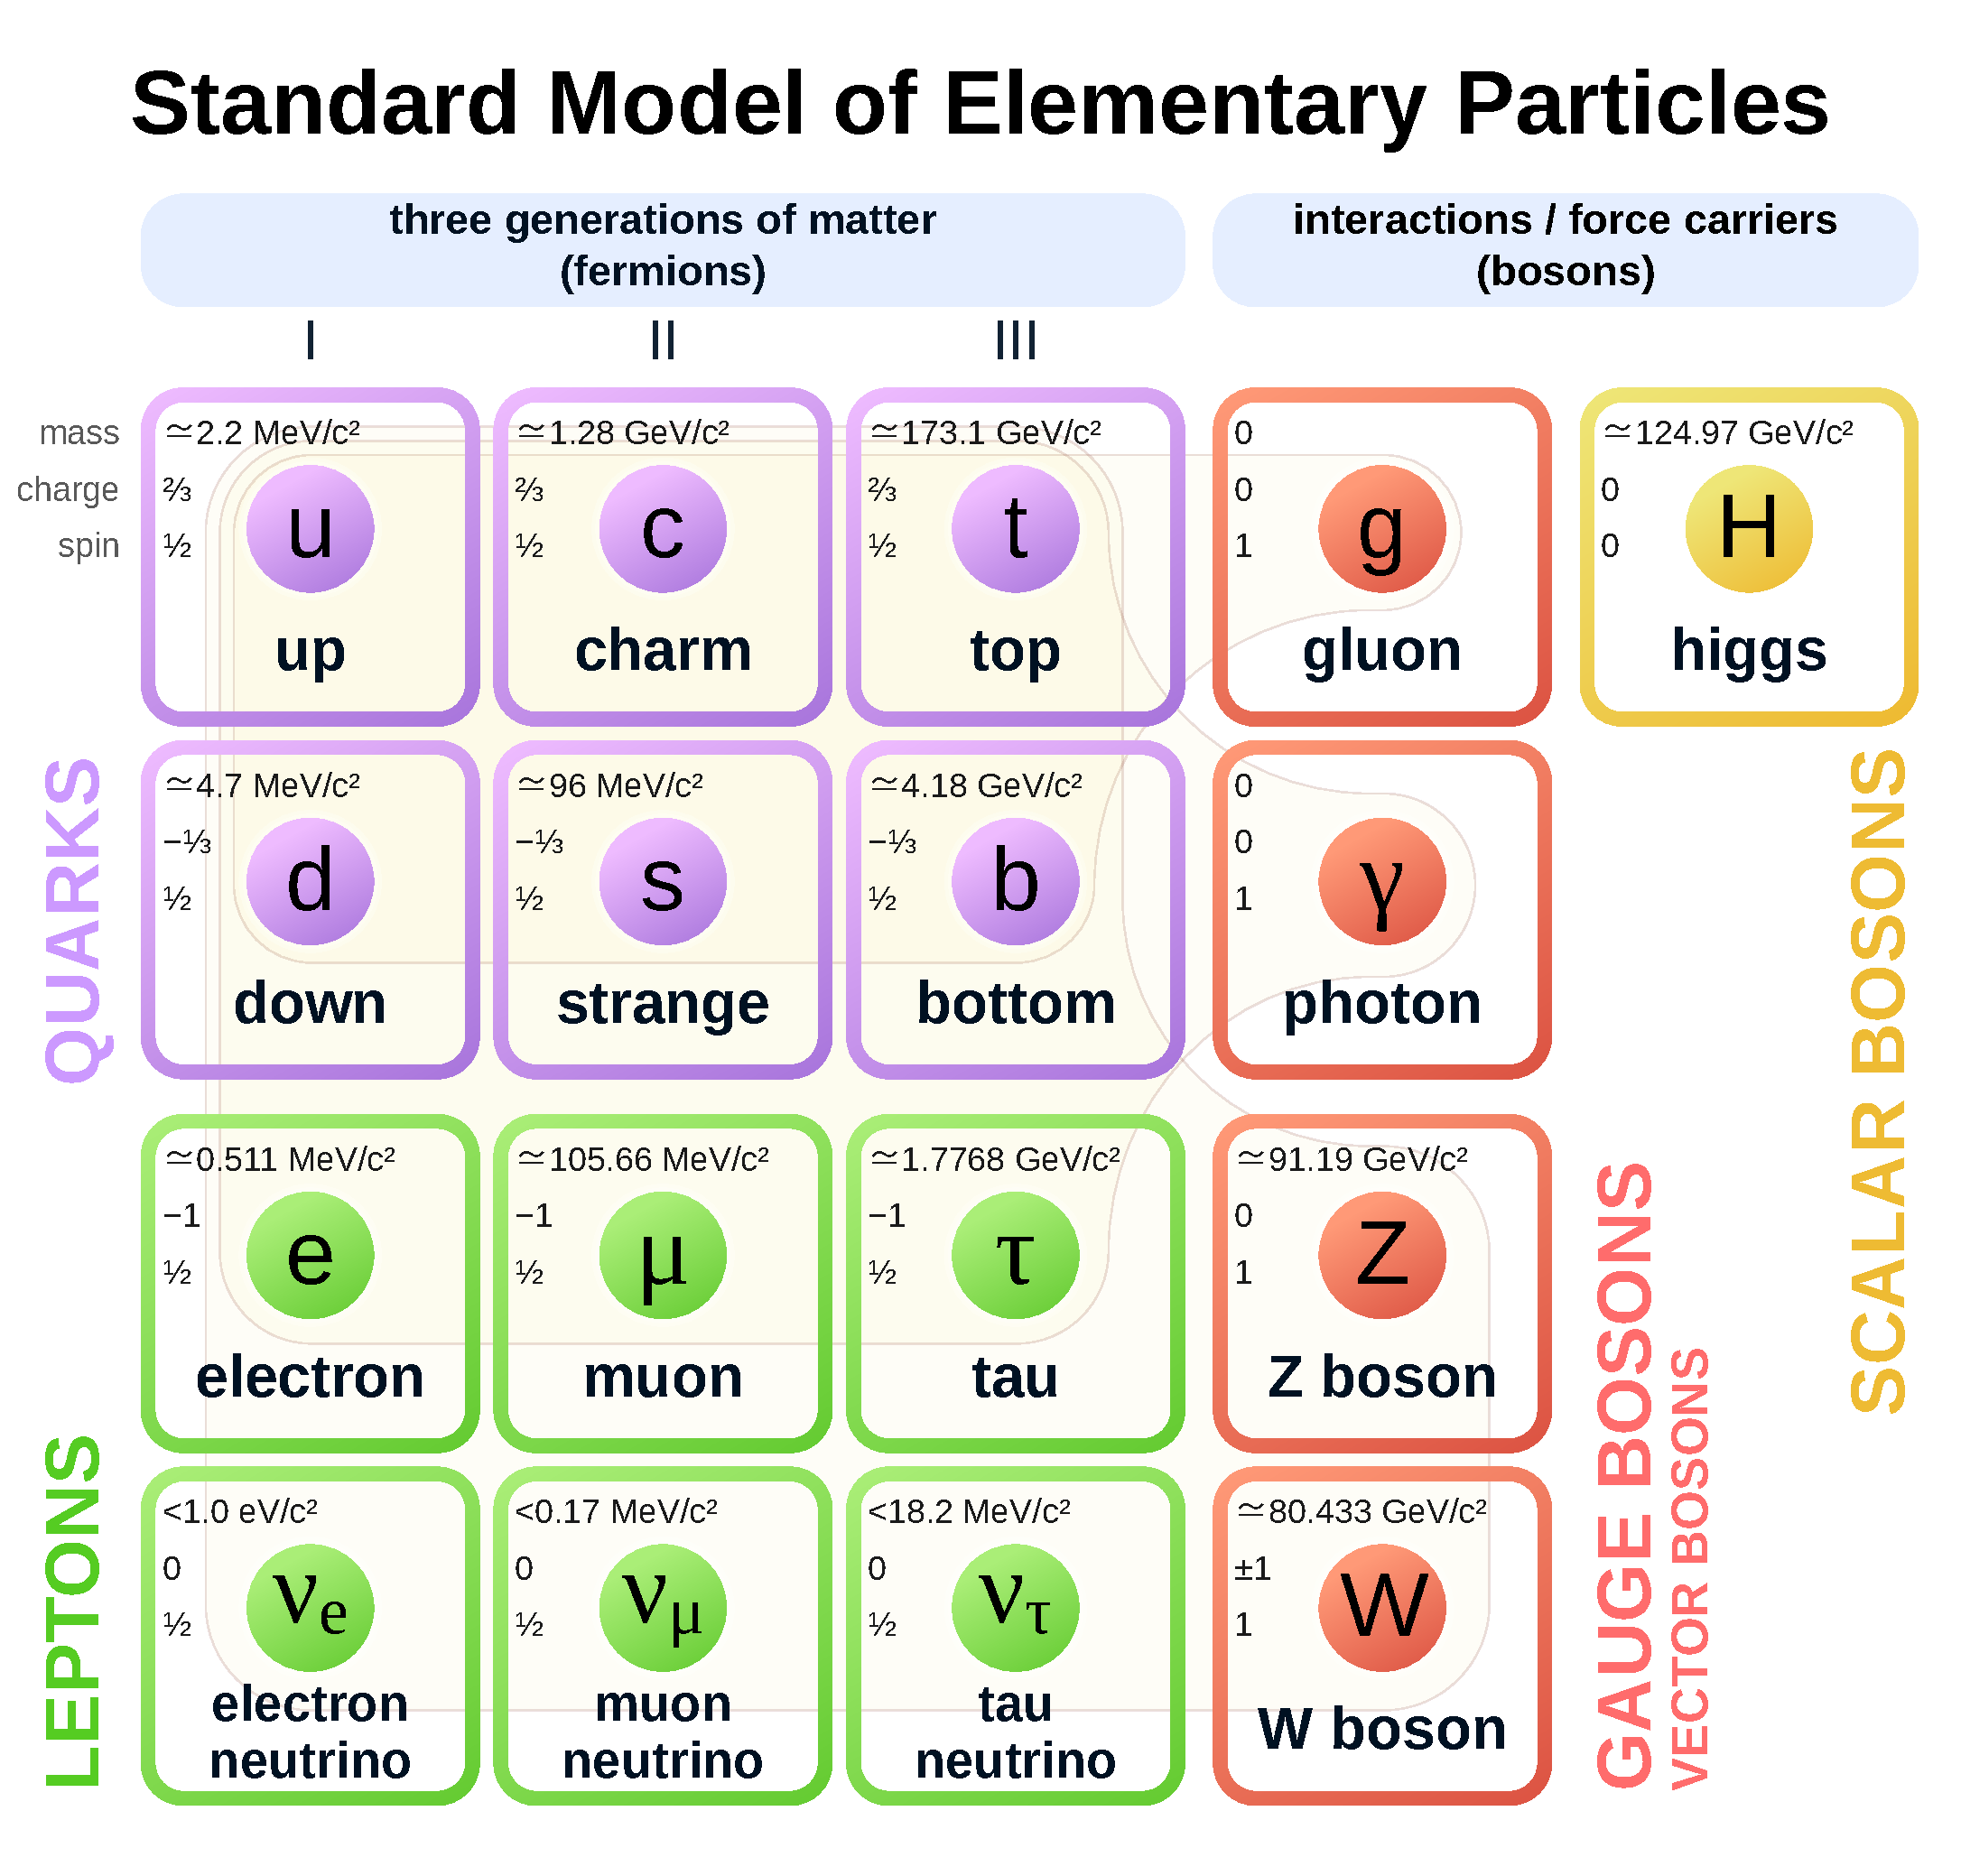
\includegraphics[width=\textwidth]{02standard_model.pdf}}
    \caption[The standard model.]{Fundamental particles in the Standard Model.
    Source: \href{https://commons.wikimedia.org/wiki/Main_Page}{Wikimedia Commons}.}
    \label{fig::10.02::standard_model}
\end{figure}
